\documentclass[times, utf8, zavrsni, numeric]{fer}
\usepackage{booktabs}
\usepackage{listings}

\begin{document}

% TODO: Navedite broj rada.
\thesisnumber{797}

% TODO: Navedite naslov rada.
\title{Rješavanje problema bojanja grafa evolucijskim algoritmom}

% TODO: Navedite vaše ime i prezime.
\author{Filip Penzar}

\maketitle

% Ispis stranice s napomenom o umetanju izvornika rada. Uklonite naredbu \izvornik ako želite izbaciti tu stranicu.
% \izvornik

% Dodavanje zahvale ili prazne stranice. Ako ne želite dodati zahvalu, naredbu ostavite radi prazne stranice.
\zahvala{}

\tableofcontents

\chapter{Uvod}
Kod NP-teških problema pretraživanja nije moguće pronaći optimalno rješenje iscrpnim pretraživanjem u realnom vremenu za velike skupove podataka. Iz tog se razloga koriste heuristički algoritmi koji uz različite pretpostavke o problemu pronalaze rješenja u prihvatljivom vremenu, smanjujući prostor pretraživanja. Upravo zbog smanjivanja prostora pretraživanja rješenja pronađena takvim algoritmima nisu uvijek optimalna.

Bojanje grafa, pronalazak njegovog kromatskog broja, je NP-težak problem određivanja minimalnog broja boja kojima se graf može obojati tako da su svaka dva susjedna vrha obojana drugom bojom. Evolucijski algoritmi su heuristički algoritmi inspirirani procesima u prirodi, a posebno su učinkoviti kod rješavanja optimizacijskih problema. Ovaj rad pobliže opisuje način rada evolucijskih algoritama, njihov podskup genetskih algoritama, problem bojanja grafa te primjenu i analizu evolucijskih algoritama pri određivanju kromatskog broja grafa.

U drugom poglavlju daje se kratko objašnjenje i uvod u problem određivanja kromatskog broja grafa. U poglavlju se analiziraju iscrpni algoritmi traženja kromatskog broja. Zatim se u trećem poglavlju objašnjava princip rada evolucijskih algoritama te se detaljnije obrađuju genetski algoritmi, njihov način rada te različite varijacije parametara i funkcija koje utječu na kvalitetu dobivenog rješenja. U četvrtom poglavlju dan je kratak pregled korištenih biblioteka i podataka. 

Peto poglavlje opisuje način određivanja kromatskog broja grafa genetskim algoritmom, implementaciju rješenja te korištene parametre i razloge njihovog odabira. U šestom se poglavlju iznose i uspoređuju rezultati testiranja različitih varijacija algoritma. Sedmo poglavlje objašnjava dobivene podatke i iznosi zaključak.

\chapter{Kromatski broj grafa}
Kromatski broj grafa, $\chi(G)$, predstavlja minimalan broj boja s kojima se mogu obojati vrhovi grafa, tako da niti jedna dva susjedna vrha (vrhovi spojeni bridom) nisu obojana istom bojom \cite{kovaceviv2020diskretna}. 

\section{Motivacija}
Problem bojanja grafa vrlo je bitan problem zbog njegove široke primjene. Kromatski broj se koristi u rješavanju mnogih problema; problema raspoređivanja, dodjele registara u procesoru, rješavanja Sudoku, dodjele radio frekvencije, sparivanje uzoraka, sinkronizacije paralelnih procesa, bojanje karata itd. Svi ovi problemi mogu se reprezentirati grafom, a njihovo rješenje bojanjem zadanog grafa. Pronalaskom kromatskog broja rješavamo problem koristeći minimalne potrebne resurse \cite{rajagaspar2022applications}. 

\begin{figure}[htb]
\centering
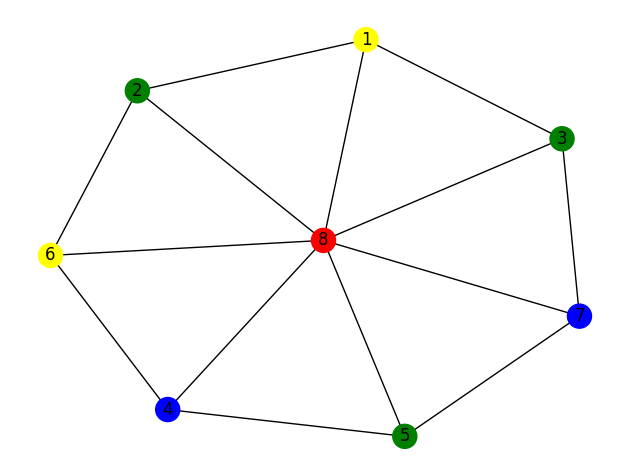
\includegraphics[width=10cm]{images/8_vertices_example.png}
\caption{Graf s osam vrhova i $\chi(G)=4$}
\label{fig:graf s obojanim vrhovima}
\end{figure}

\section{Određivanje kromatskog broja}
Pronalazak kromatskog broja grafa je NP-težak problem, što znači da je vremenska složenost njegovog pronalaska eksponencijalna \cite{shen2003solving}. Zbog toga nije praktično koristiti se algoritmima iscrpnog pretraživanja na grafovima s većim brojem vrhova.

\subsection{Iscrpno pretraživanje}
Jednostavan algoritam isrcpnog pretreaživanja prošao bi sve kombinacije $k$ boja i $n$ vrhova; njegova vremenska složenost je $O(k^n)$. Implementacija iscrpnog algoritma određivanja kromatskog broja rekurzijom u programskom jeziku Python dana je slikom \ref{fig:algoritam iscrpnog pretraživanja}.

\begin{figure}[htb]
\centering
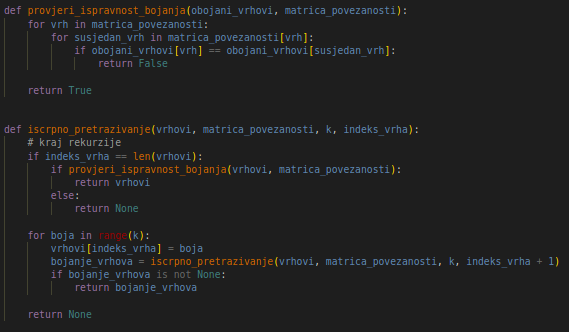
\includegraphics[width=12cm]{images/iscrpno_pretrazivanje.png}
\caption{Algoritam iscrpnog pretraživanja}
\label{fig:algoritam iscrpnog pretraživanja}
\end{figure}

Jedan iterativni pristup pronalaska kromatskog broja je pokušati obojati graf s $k=n$ boja, gdje je $n$ broj vrhova. Ukoliko uspijemo pronaći takvo rješenje, pokušavamo s $k=n-1$ bojom \cite{geeksforgeeks}. Postupak nastavljamo sve do koraka $m: (m < n)$ kada više ne pronalazimo ispravno bojanje. Tada zaključujemo da je $\chi(G)=k=n-m+1$. Algoritam je prikazan slikom \ref{fig:algoritam iterativnog iscprnog odredivanja kromatskog broja}.

\begin{figure}[htb]
\centering
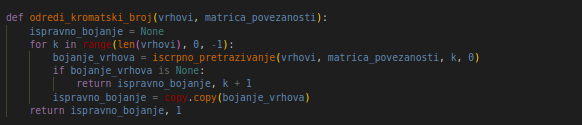
\includegraphics[width=12cm]{images/iterativni_algoritam_iscprnog_pretrazivanja.png}
\caption{Iterativno određivanje kromatskog broja s iscrpnim pretraživanjem}
\label{fig:algoritam iterativnog iscprnog odredivanja kromatskog broja}
\end{figure}

\subsection{Pohlepno pretraživanje}
Pohlepan algoritam kreće od vrha s najvećim stupnjem, onim s najviše susjednih vrhova. Njega boja prvom dostupnom bojom. Zatim pokušava obojati sljedeći vrh s najvećim stupnjem, uzimajući prvu boju s kojom može legalno obojati taj vrh, tako da je različite boje od njemu susjednih vrhova. Postupak se ponavlja do zadnjeg vrha, ili do kad više nema dostupnih boja \cite{cranston2015brooks}. Složenost ovakvog algoritma je $O(n^2)$, jer za svaki vrh mora proći po svim dotad obojanim vrhovima i vidjeti kojim bojama može obojati trenutni vrh. Ovakvo pretraživanje ne daje uvijek rješenje kad ono postoji, no prednost mu je što je manje vremenske složenosti od iscrpnog pretraživanja. Algoritam je dan slikom \ref{fig:pohlepno pretrazivanje}.

\begin{figure}[htb]
\centering
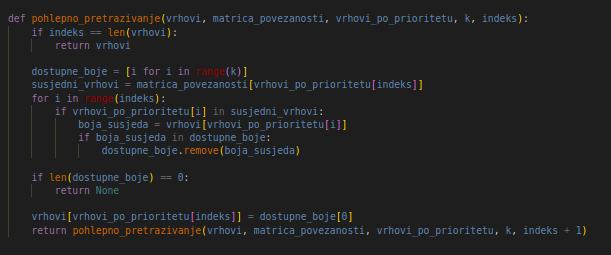
\includegraphics[width=12cm]{images/pohlepni_algoritam.png}
\caption{Pohlepno pretraživanje}
\label{fig:pohlepno pretrazivanje}
\end{figure}


\subsection{Usmjereno iscrpno pretraživanje}
Algoritam usmjerenog iscrpnog pretraživanja radi vrlo slično kao i pohlepno pretraživanje, uz bitnu preinaku da ukoliko ne pronađe legalno bojanje, traži dalje. Algoritam odredi moguće boje za bojanje trenutnog vrha kao i pohlepni algoritam, ali ukoliko ne uspije obojati graf s prvom bojom, proba s drugom mogućom, pa trećom i tako dalje. Ovakav će algoritam uvijek pronaći ispravno bojanje i upravo će to bojanje biti ono s minimalnim brojem boja, odnosno kromatski broj grafa. Algoritam je dan slikom \ref{fig:iscrpno usmjereno pretrazivanje}.

\begin{figure}[htb]
\centering
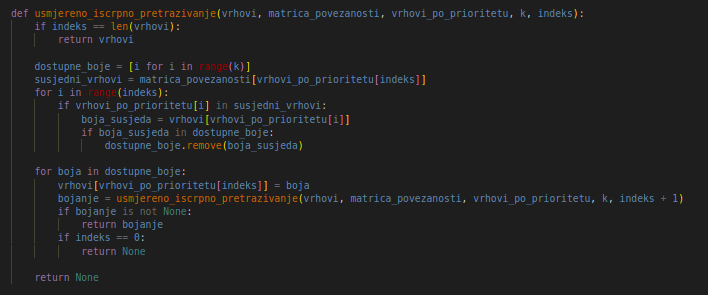
\includegraphics[width=12cm]{images/iscrpno_usmjereno_pretrazivanje.png}
\caption{Usmjereno iscrpno pretraživanje}
\label{fig:iscrpno usmjereno pretrazivanje}
\end{figure}

Svaki graf s $n$ vrhova možemo obojati s $n$ boja, no uvjet na gornju ogradu kromatskog broja možemo postrožiti.

\section{Gornja ograda na kromatski broj}
Prema Brookovom teoremu, kromatski broj svakog grafa je maksimalno $\Delta$ + 1, gdje je $\Delta$ maksimalan stupanj grafa \cite{cranston2015brooks}. 

Maksimalan stupanj grafa, $\Delta$, je najveći broj bridova koji su incidentni s bilo kojim pojedinačnim vrhom u grafu.

\section{Donja ograda na kromatski broj}
Donja ograda na kromatski broj je 1. Ovo se postiže samo za grafove u kojima niti jedna dva vrha nisu međusobno povezana.

\begin{figure}[htb]
\centering
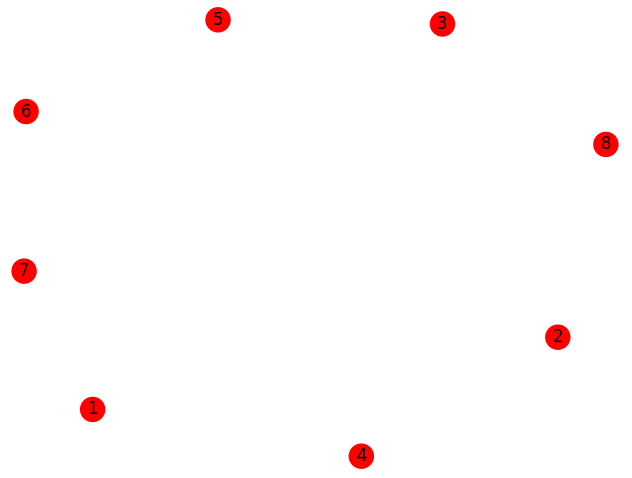
\includegraphics[width=10cm]{images/8_vertices_nepovezane.png}
\caption{Graf s $\chi(G)=1$}
\label{fig:graf s kromatskim brojem 1}
\end{figure}

\chapter{Evolucijski algoritmi}

Evolucijski algoritmi su algoritmi koji inspiraciju vuku iz prirode, iz Darwinonve teorije evolucije. Probleme rješavaju kroz procese koji emuliraju ponašanje živih bića i sustava u prirodi.

Rješenja problema u evolucijskim algoritmima predstavljaju pojedine jedinke unutar populacije. Populacija je na početku određena slučajno, a kasnije kroz naraštaje, odnosno iteracije algoritma, bolja rješenja preživljavaju i reproduciraju se, dok se lošija rješenja miču, izumiru. Ovime je osigurano da su jedinke novog naraštaja potomci najboljih jedinki prethodnog naraštaja čime se postiže konvergencija prema optimalnom rješenju \cite{cupic2010prirodom}.

Evolucijski algoritmi odlični su kod pronalaženja rješenja za optimizacijske probleme. Kroz naraštaje, pojedina rješenja postaju sve bolja i bliža optimalnom. Bitno je imati na umu da su evolucijski algoritmi podskup heurističkih algoritama, što znači da pronađena rješenja nisu nužno optimalna. Uzrok tome je što se ne pretražuje cijeli prostor već samo njegov podskup koji je ograničen početnom populacijom i parametrima evolucijskog algoritma, određenima na temelju neke heuristike.

\section{Genetski algoritmi}
Genetski algoritmi podskup su Evolucijskih algoritama. Jedinke, rješenja, kodirana su u obliku genoma. Iz početne populacije jedinki biraju se one najbolje pomoću funkcije dobrote (eng. \textit{fitness}) ili pomoću funkcije cijene (eng. \textit{cost}) koje će biti roditelji novoj generacije. Iz genoma odabranih roditelja se pomoću procesa križanja određuju genomi djece. Osim procesa križanja i odabira roditelja, važnu ulogu igraju i mutacije gena na genomu. Proces mutacije događa se nakon križanja roditelja, kada se s određenom vjerojatnošću ili heuristikom mijenjaju neki od gena na genomu. Mutacije su bitne jer se njima proširuje prostor pretraživanja, uvode nove varijacije rješenja te se sprječava ostanak u području lokalnog optimuma rješenja \cite{cupic2010prirodom}.

\subsection{Kodiranje genoma}
Genom (kromosom) u sklopu Genetskih algoritama predstavlja jedan specifičan organizam, odnosno jedno moguće rješenje. Genom se sastoji od vektora gena. Svaki gen može poprimiti određenu vrijednost. Za ispravan rad genetskog algoritma nužno je pravilno kodirati rješenja u obliku genoma.

Kod problema bojanja grafa, genom je vektor od $n$ elemenata gdje je $n$ broj vrhova u grafu. Vrijednost svakog gena je iz skupa od $k$ elemenata, gdje $k$ predstavlja broj različitih boja \cite{marappan2013new}. Konačno rješenje je vektor u kojemu su elementi pobojani s $k$ različitih boja tako da pripadajući spojeni vrhovi nemaju istu vrijednost. Ukoliko su dva vrha spojena i obojana su istom bojom, takvu jedniku ne smatramo rješenjem problema. Na slici \ref{fig:kodirani genom} prikazan je genom jedne jedinke koja je optimalno rješenje bojanja grafa na slici \ref{fig:kodiranje genoma graf}.

\begin{figure}[htb]
\centering
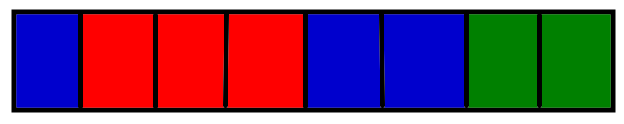
\includegraphics[width=8cm]{images/genom_encoding.png}
\caption{Vektor gena - genom, $k=3$, $n=8$}
\label{fig:kodirani genom}
\end{figure}

\begin{figure}[htb]
\centering
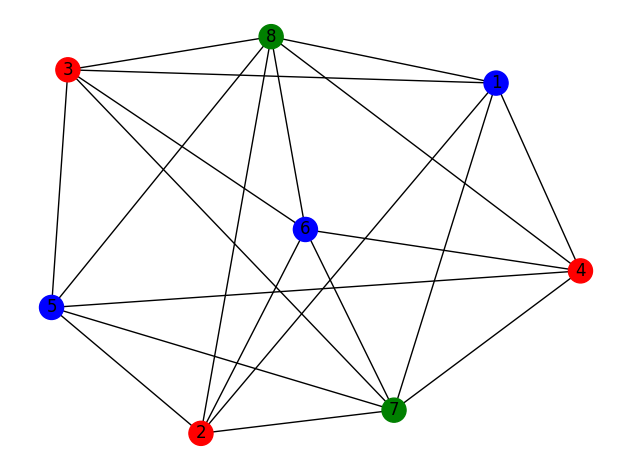
\includegraphics[width=10cm]{images/genom_encoding_graph.png}
\caption{Pripadajući obojani graf, $\chi(G)=3$}
\label{fig:kodiranje genoma graf}
\end{figure}

\subsection{Funkcija cijene}
\label{sec:funkcija cijene}
Određivanje koliko je koja jedinka dobra određuje se pomoću funkcije cijene. Ona mjeri koliko je trenutno rješenje udaljeno od ciljnog. Što je cijena jedinke manja, to je rješenje bolje. Kada cijene neke jedinke dosegne 0, pronađeno je ispravno rješenje.

Suprotno funkciji cijene je funkcija dobrote, prema kojoj bolje jedinke imaju veću vrijednost.

U primjeru bojanja grafova, ciljno rješenje ne smije imati niti jedna dva susjedna vrha obojana istom bojom. Za svaka dva krivo spojena vrha, funkcija cijene raste za jedan \cite{geeksforgeeks}. Implementacija algoritma prikazana je slikom \ref{fig:funkcija cijene}.

\begin{figure}[htb]
\centering
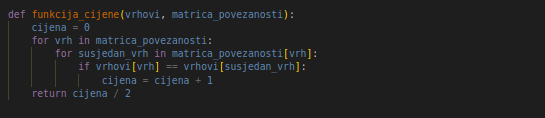
\includegraphics[width=12cm]{images/funkcija_cijene.png}
\caption{Funkcija cijene implementirana u Pythonu}
\label{fig:funkcija cijene}
\end{figure}

\subsection{Određivanje roditelja}
Roditelji se iz populacije biraju na temelju njihove izračunate cijene. Jedinke s manjom cijenom imaju prednost pri reproduciranju nad jedinkama s većom cijenom. Postoji mnogo različitih strategija odabira roditelja u sklopu genetskih algoritama, a neke od njih su:
\begin{itemize}
    \item Slučajna selekcija
    \item Selekcija stabilnog stanja
    \item Roullete wheel
    \item Rang selekcija
\end{itemize}

\subsubsection{Slučajna selekcija}
Kao naivnu metodu selekcije roditelja koristi se Slučajna selekcija. Iz populacije se slučajnim odabirom izabiru dvije jedinke kao roditelji novoj jedinci. Ova metoda je manje uspješna od ostalih metoda selekcije i zato nije pretjerano korištena. Razlog manjoj uspješnosti je što cijena izračunata za pojedine jedinke nimalo ne utječe na izbor jedinke kao roditelja. Bolje jedinke nemaju nikakvu prednost kod reprodukcije što znači da rješenja sporije konvergiraju, ili uopće ne konvergiraju k optimumu.

\subsubsection{Selekcija stabilnog stanja}
Kod selekcije stabilnog stanja (\textit{eng. Steady State Selection}), među populacijom se biraju dvije jedinke s najboljom dobrotom. Iz njih se stvaraju dvije nove jedinke, njihova djeca, i na njima se provodi mutacija. Zatim se izračunava dobrota djece i djeca se dodaju populaciji. Iz populacije se tada izbacuju dvije jednike s najmanjom dobrotom. Ovakav pristup odabira roditelja i njihove djece proizvodi svega dvije nove jedinke po generaciji, ali su one uvijek potomci dvoje roditelja s najboljom dobrotom.  

\subsubsection{Roullete wheel}
Nakon što su izračunate cijene za sve jedinke u generaciji, svakoj se pridjeljuje udio na \textit{roullete wheel-u}. Udio je proporcionalan cijenama jedinki; one s nižom cijenom (većom dobrotom) će imati veći udio na \textit{roullete wheel-u}. Time se osigurava da bolje jedinke imaju veću vjerojatnost da budu odabrane kao roditelji sljedećoj generaciji. Rješenje se tako brže približava optimumu jer će djeca naslijediti gene od uspješnijih roditelja. 

\begin{figure}[htb]
\centering
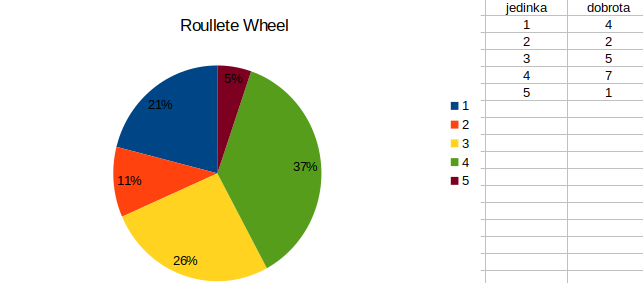
\includegraphics[width=14cm]{images/roullete_wheel_selection.png}
\caption{Primjer \textit{roullete wheel-a}}
\label{fig:roullete wheel}
\end{figure}

Nedostatak ove metode je što se može dogoditi da neka jedinka bude nesrazmjerno dobra u odnosu na druge jedinke, ali vodi samo lokalnom optimumu. Algoritam će tada odabrati takvu jedinku kao roditelja i sva njezina djeca će posljedično biti relativno uspješna, ali neće konvergirati optimalnom rješenju.

\subsubsection{Rang selekcija}
Rang selekcija po principu je slična \textit{roullete wheel-u}, ali se umjesto proporcionalnog udjela vjerojatnosti prema cijeni, jedinke prvo rangiraju prema cijeni, a udjeli na kotaču se zatim dodjeljuju proporcionalno rangu.

\begin{figure}[htb]
\centering
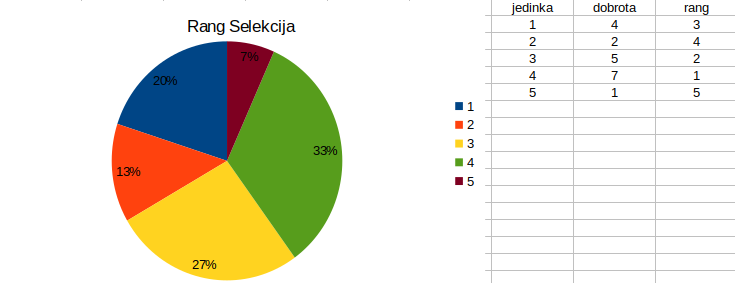
\includegraphics[width=14cm]{images/rang_selekcija.png}
\caption{Primjer rang selekcije}
\label{fig:rang selekcija}
\end{figure}

Na taj način svaki rang uvijek ima jednaku vjerojatnost biti izabran. Bolje jedinke imaju veću vjerojatnost biti izabrane kao roditelji sljedećoj generaciji, a ne može se dogoditi da neke jedinke koje vode do lokalnog optimuma imaju preveliku prednost nad ostalim jedinkama te da zbog toga algoritam ne konvergira u globalno rješenje.

\subsection{Križanje}
Križanje je postupak kojim se iz izabranih genoma roditelja dobiva genom potomka. Potomak se sastoji od pomješanog genoma svojih roditelja. Križanje se izvodi tako da se na slučajnom mjestu prerežu genomi oba roditelja u točki prijeloma, zamijene se prvi dijelovi genoma i dobiju se dvije nove jedinke; prva jedinka s prvim dijelom genoma od prvog roditelja i drugim dijelom genoma od drugog roditelja, i druga jedinka s prvim dijelom genoma od drugog roditelja i drugim dijelom genoma od prvog roditelja. Osim križanja sa samo jednom točkom prijeloma, postoji i križanje s više točaka prijeloma. 

Postupak križanja vizualno je prikazan na slikama \ref{fig:kromosomi roditelja}, \ref{fig:krizanje}, \ref{fig:kromosomi djece}.

\begin{figure}[htb]
\centering
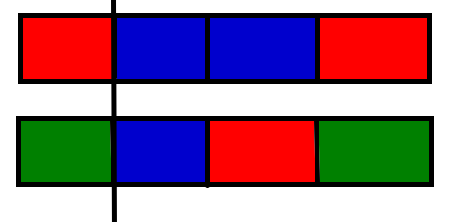
\includegraphics[width=4cm]{images/kromosomi_roditelja.png}
\caption{Kromosomi roditelja}
\label{fig:kromosomi roditelja}
\end{figure}

\begin{figure}[htb]
\centering
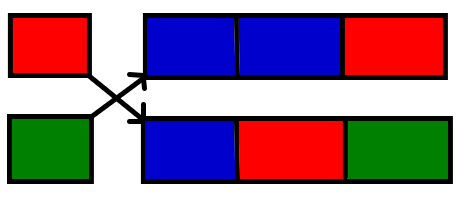
\includegraphics[width=4cm]{images/krizanje.png}
\caption{Križanje}
\label{fig:krizanje}
\end{figure}

\begin{figure}[htb]
\centering
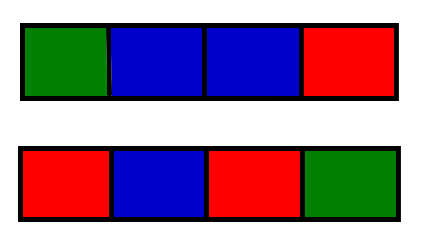
\includegraphics[width=4cm]{images/kromosomi_djece.png}
\caption{Kromosomi djece}
\label{fig:kromosomi djece}
\end{figure}

Ukoliko smo koristili dobru metodu za odabir roditelja, djeca će se sastojati od pomiješanih gena uspješnih roditelja, približiti će se optimumu. Često se dogodi da su djeca manje dobrote od svojih roditelja, no prosječno gledano na cijeloj populaciji, dobrota djece se povećava.

\subsection{Mutacije}
Mutacije su promjene gena na kromosomima jedinki. One su vrlo bitne u genetskim algoritmima jer nam omogućuju da pretražujemo rješenje na širem prostoru. Ukoliko ne bismo uveli mutacije na genima, geni početne populacije bi u potpunosti određivali mogući prostor pretraživanja. Sve nove jedinke mogle bi biti jedino kombinacije početnog skupa gena. Mutacije također ubrzavaju pretraživanje prostora, jer će neke jedinke "odskočiti" od trenutne populacije, uvesti novinu u naš skup jedinki. Ukoliko su mutacije nepovoljne, takve jedinke imati će manju dobrotu, neće se uspješno razmnožavati i takva mutacija će izumrijeti. Pozitivne će mutacije s druge strane, povećati dobrotu jedinke i tako povećati vjerojatnost reprodukcije jedinke s takvim genom. Gen će se dalje propagirati i dovesti cijelu populaciju bliže optimumu.

Slika \ref{fig:kromosom prije mutacije} prikazuje kromosom prije mutacije, a slika \ref{fig:kromosom poslije mutacije} kromosom poslije mutacije na trećem i osmom genu.

\begin{figure}[htb]
\centering
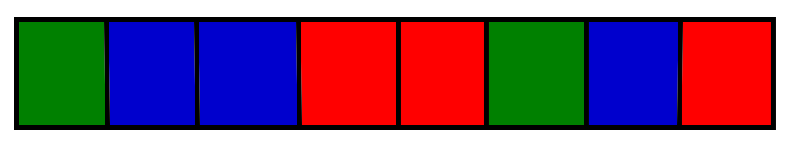
\includegraphics[width=4cm]{images/prije_mutacije.png}
\caption{Kromosom prije mutacije}
\label{fig:kromosom prije mutacije}
\end{figure}

\begin{figure}[htb]
\centering
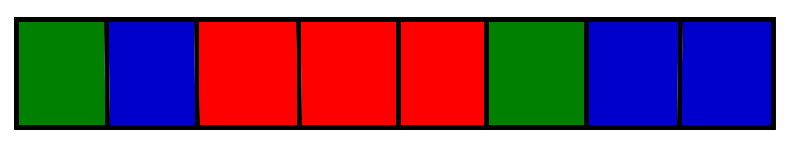
\includegraphics[width=4cm]{images/poslije_mutacije.png}
\caption{Kromosom poslije mutacije}
\label{fig:kromosom poslije mutacije}
\end{figure}

Klasično se mutacije implementiraju tako da svaki gen ima nezavisnu vjerojatnost mutacije. Mutacija se provodi nakon križanja. Kod nekih specifičnih problema, poput bojanja grafa, bolje rezultate daju usmjere mutacije na genima koje ovise o trenutnom stanju svih gena jedinke.

\section{Implementacija genetskog algoritma}
Nakon slučajnog izbora početne populacije, nad svakom jedinkom izračunava se njezina dobrota. Na temelju dobrote se odabiru roditelji nove generacije. Roditelji se križaju, a zatim se nad dobivenom djecom izvode mutacije. Djeca zamjenjuju roditelje u populaciji. Ovaj se postupak ponavlja sve dok se ne postigne željena dobrota, pronađe optimalno rješenje problema ili se ne pređe određen broj iteracija. Pseudokod genetskog algoritma dan je slikom \ref{fig:pseudokod genetskog algoritma}.

\begin{figure}[htb]
\centering
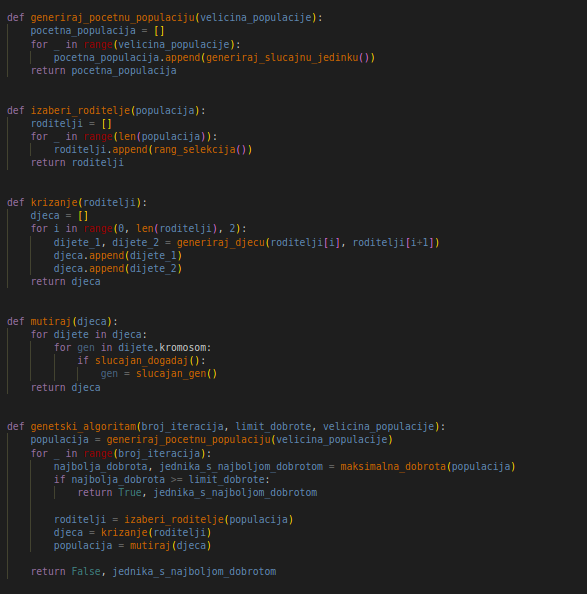
\includegraphics[width=14cm]{images/genetski_algoritam_pseudokod.png}
\caption{Pseudokod genetskog algoritma}
\label{fig:pseudokod genetskog algoritma}
\end{figure}

\chapter{Korištene biblioteke i podaci}

\section{PyGAD}
PyGAD je biblioteka otvorenog koda za programski jezik Python pomoću koje se vrlo jednostavno mogu izgraditi modeli genetskih algoritama. Biblioteka dolazi s mnoštvom ugrađenih metoda, specifičnima za genetske algoritme. PyGAD je vrlo fleksibilan i dozvoljava definiranje vlastitih funckija izračuna dobrote, izbora roditelja, križanja i mutacije.

\subsection{Instalacija}
Instalacija biblioteke vrši se preko PIP-a sljedećom naredbom:

\begin{lstlisting}[language=bash]
  $ pip install pygad
\end{lstlisting}

\section{NetworkX}
NetworkX je Python paket za stvaranje, rukovanje i proučavanje strukture, dinamike i funkcija složenih mreža. U sklopu ovog projekta korišten je kod vizualizacije grafova te njihovog bojanja.

\subsection{Instalacija}
Instalacija biblioteke vrši se preko PIP-a sljedećom naredbom:

\begin{lstlisting}[language=bash]
  $ pip install networkx[default]
\end{lstlisting}

\section{House of Graphs}
\label{sec:house of graphs}
House of Graphs \cite{houseofgraphs} je Web-stranica koja sadržava bazu grafova s karakteristikama koja dozvoljava njihovo besplatno preuzimanje. House of Graphs razvijen je u suradnji sveučilišta Ghent i sveučilišta KU Leuven.

U sklopu projekta preuzeti su grafovi s brojem vrhova između 1 i 250. Za svaki od grafova definirana je matrica susjedstva kao i kromatski broj grafa. Na taj se način rješenje dobiveno genetskim algoritmom moglo usporediti sa stvarnom vrijednošću kromatskog broja grafa. Za neke od kompleksnijih grafova nije izračunat kromatski broj (\textit{Chromatic number: Computation timeout}) te su takvi grafovi preskočeni kod izračuna točnosti rada genetskog algoritma.

\begin{figure}[h]
\centering
\begin{minipage}{.5\textwidth}
  \centering
  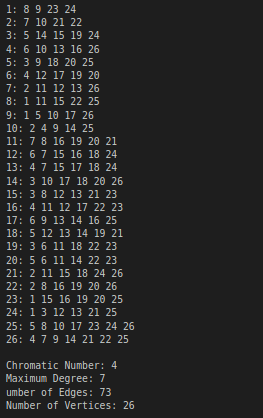
\includegraphics[width=5cm]{images/26_vertices_graph_definition.png}
  \caption{Definicija grafa s 26 vrhova}
  \label{fig:definicija grafa s 26 vrhova}
\end{minipage}%
\begin{minipage}{.5\textwidth}
  \centering
  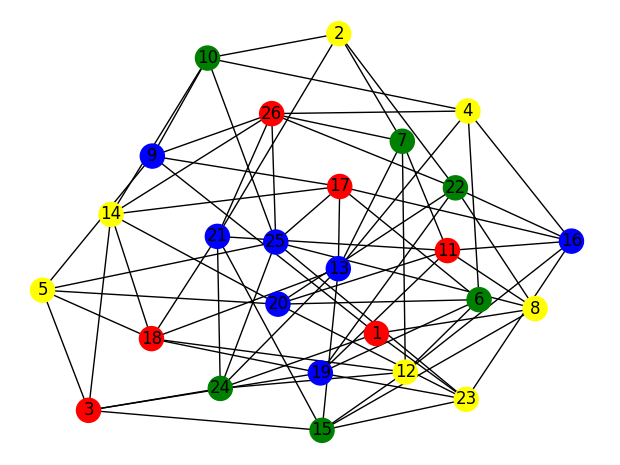
\includegraphics[width=8cm]{images/26_vertices_graph.png}
  \caption{Bojanje grafa s 26 vrhova s 4 boje}
  \label{fig:obojani graf s 26 vrhova}
\end{minipage}
\end{figure}

Definicija grafa preuzetog s House of Graphs Web-stranice s 26 vrhova dana je slikom \ref{fig:definicija grafa s 26 vrhova}, a ispravno bojanje za taj graf dano je slikom \ref{fig:obojani graf s 26 vrhova}.


\chapter{Praktični dio}
Projekt je pisan u programskom jeziku Python. Python je izabran zbog jednostavnosti korištenja i dobre potpore rješavanju problema u obliku slobodno dostupnih biblioteka.

\section{Određivanje dobrote jedinki}
Funkcija cijene korištena u sklopu projekta opisana je u potpoglavlju \ref{sec:funkcija cijene}. Funkcija je prilagođena kako bi bila kompatibilna s PyGAD bibliotekom koja zahtjeva korištenje funkcije dobrote. Kod određivanja ispravnog bojanja grafa prirodno je koristiti funkciju cijene, kao mjeru broja vrhova obojanih krivom bojom. Ispravno bojanje grafa određeno je maksimumom funkcije dobrote koji je nula (niti jedan vrh nije obojan istom bojom kao i njegov susjed), a za svaki krivo obojani vrh dobrota pada za jedan. Lošije jedinke tako imaju manju dobrotu.

\section{Određivanje roditelja}
Roditelji su određivani na tri načina; slučajnim odabirom, rang selekcijom i selekcijom stabilnog stanja. Slučajan odabir izabran je kako bi se pokazali nedostatci te metode, ali i dao uvid u rad ostatka algoritma i odabira ostalih parametara. Rang selekcija i selekcija stabilnog stanja korištene su kako bi se postigli optimalni rezultati.

\section{Križanje}
Za metodu križanja je korišteno križanje s jednom točkom prijeloma.

\section{Mutacije}
Najbitniju ulogu u samom algoritmu imale su mutacije. Na početku su se koristile slučajne mutacije s vjerojatnošću mutiranja na svakom genu od 20\%. Ovaj relativno visok postotak uzet je kako bi se populacija brže širila po prostoru pretraživanja te ne bi zapela u lokalnim optimumima \cite{geeksforgeeks}. Problem je što geni unutar svake jedinke nisu nezavisni, pa se na slijepo pogađanje nisu dobili zadovoljavajući rezultati. Iz tog razloga isprobane su i neke kompleksnije funkcije mutacije. 

\subsection{Slučajna mutacija na krivim vrhovima}
\label{sec: slucajna mutacija na krivim vrhovima}
Prvi pristup mutaciji slučajno je mijenjao vrijednosti samo onih gena koji su obojani istom bojom kao i njihovi susjedi. Na ovaj način su vrhovi koji su bili dobro obojani ostali netaknuti. Rješenje na ovaj način konvergira prema pravom jer se jednom pronađena dobra bojanja ne mijenjaju. Slučajna mutacija na krivim vrhovima ne uzima u obzir njihove susjede kod odabira nove boje. Zbog toga se prostor pretraživanja pretražuje na relativno širokom području \cite{hindi2012genetic}. Implementacija je dana u Pythonu slikom \ref{fig:slucajna mutacija na krivim vrhovima}.

\begin{figure}[htb]
\centering
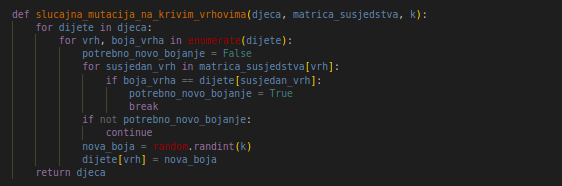
\includegraphics[width=14cm]{images/slucajna_mutacija_na_krivim_vrhovima.png}
\caption{Slučajna mutacija na krivim vrhovima}
\label{fig:slucajna mutacija na krivim vrhovima}
\end{figure}

\subsection{Ciljana mutacija na krivim vrhovima}
\label{sec: ciljana mutacija na krivim vrhovima}
U ovoj metodi, slično kao i u potpoglavlju \ref{sec: slucajna mutacija na krivim vrhovima}, mutacija se odvija samo na vrhovima koji su obojani isto kao i neki od njihovih susjeda. Mutacija na takvim vrhovima nije slučajna, već se gledaju susjedi takvog vrha i za njegovo ponovno bojanje bira se boja kojom njegovi susjedi nisu obojani. Ukoliko takva boja ne postoji, slučajnim odabirom izabire se neka od boja iz skupa svih boja. Ovakva implementacija osigurava da dobro obojani vrhovi ostanu netaknuti, a oni krivo obojani ciljano promijene svoju boju ne narušavajući ispravna bojanja ostalih vrhova ukoliko to mogu \cite{hindi2012genetic}. Implementacija je dana u Pythonu slikom \ref{fig:ciljana mutacija na krivim vrhovima}.

\begin{figure}[htb]
\centering
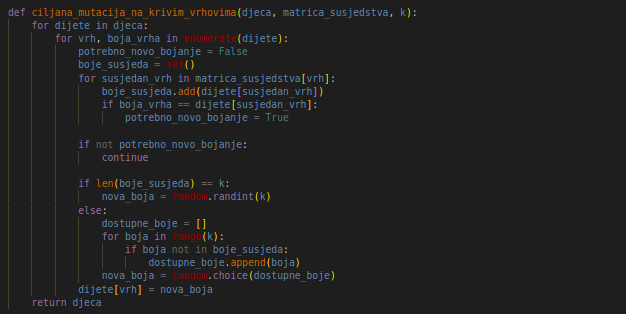
\includegraphics[width=14cm]{images/ciljana_mutacija_na_krivim_vrhovima.png}
\caption{Ciljana mutacija na krivim vrhovima}
\label{fig:ciljana mutacija na krivim vrhovima}
\end{figure}

\subsection{Kombinacija slučajne i ciljane mutacije na krivim vrhovima}
\label{sec: kombinacija slucajne i ciljane mutacije na krivim vrhovima}
Ovisno o dobroti najbolje jedinke iz prethodne populacije, ovaj algoritam bira jednu od mutacija iz potpoglavlja \ref{sec: slucajna mutacija na krivim vrhovima} i potpoglavlja \ref{sec: ciljana mutacija na krivim vrhovima}. Ukoliko je dobrota najbolje jedinke blizu optimalne, nula, tada se koristi \textit{Slučajna mutacija na krivim vrhovima} jer se želi izbjeći zaustavljanje u lokalnom optimumu. Kada je dobrota najbolje jedinke daleko od optimalne, koristi se \textit{Ciljana mutacija na krivim vrhovima} jer se želi usmjerenije pretražiti prostor i na taj način stići do optimuma \cite{hindi2012genetic}. Implementacija je dana u Pythonu slikom \ref{fig:kombinacija slucajen i ciljane mutacije}.

\begin{figure}[htb]
\centering
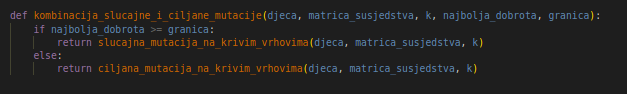
\includegraphics[width=14cm]{images/kombinacija_slucajne_i_ciljane_mutacije.png}
\caption{Kombinacija slučajne i ciljane mutacije na krivim vrhovima}
\label{fig:kombinacija slucajen i ciljane mutacije}
\end{figure}

\section{Ostali parametri}
Ostali korišteni parametri dani su tablicom \ref{tbl:ostali parametri genetrskog algoritma}.

\begin{table}[htb]
\caption{Ostali parametri genetskog algoritma}
\label{tbl:ostali parametri genetrskog algoritma}
\centering
\begin{tabular}{llr} \hline
Parametar & Vrijednost\\ \hline
broj generacija & 1000 \\
jedinke po generaciji & 50 \\
elitizam & istina \\
broj gena & $n$ \\ \hline
\end{tabular}
\end{table}

Broj generacija i broj jedinki po generaciji odabrani su kao kompromis između vremena izvođenja algoritma i uspješnosti algoritma \cite{hindi2012genetic}. Broj gena odgovara broju vrhova, $n$, jer se svaki vrh kodira svojim genom. 

Elitizam je strategija evolucijskih algoritama kojom se najbolje jedinke, u kontekstu ovog projekta jedna, automatski prenose u sljedeću generaciju. Na taj način se čuvaju uspješne jedinke, imaju više potomaka i algoritam brže konvergira optimalnom rješenju. 

\section{Postupak određivanja kromatskog broja}
Nakon parsiranja grafova preuzetih s House of Graphs (potpoglavlje \ref{sec:house of graphs}), za svaki od grafova određuje se kromatski broj. Početna vrijednost $k$ je postavljena na $\Delta + 1$. Ako se genetskim algoritmom pronašlo ispravno bojanje sa zadanim $k$ (dobrota neke jedinke je jednaka nuli), $k$ se smanjuje za 1, a najbolja jedinka se pohranjuje. Algoritam prekida s radom u dva slučaja; ukoliko je pronašao ispravno bojanje s $k=\chi(G)$ (točan kromatski broj je zadan zajedno s definicijom grafa) ili algoritam nije pronašao ispravno bojanje za trenutni $k$. U potonjem slučaju algoritam vraća $k+1$ kao zadnji ispravan broj boja. Implementacija je dana u Pythonu slikom \ref{fig:odredivanje kromatskog broja genetskim algoritmom}.

\begin{figure}[htb]
\centering
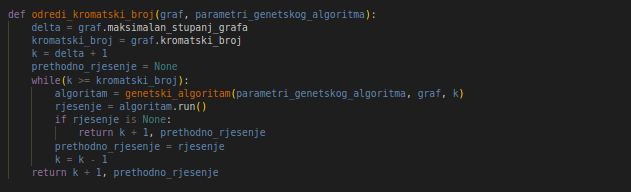
\includegraphics[width=14cm]{images/genetski_algoritam_i_odredivanje_broja.png}
\caption{Određivanje kromatskog broja genetskim algoritmom}
\label{fig:odredivanje kromatskog broja genetskim algoritmom}
\end{figure}

\section{Vizualizacija rezultata}
Podaci o uspješnom pronalasku kromatskog broja se pohranjuju, tako da je na kraju izvođenja programa moguće odrediti postotak uspješnih pronalazaka kromatkog broja. Uz to, program je u mogućnosti vizualizirati dobivene rezultate crtanjem obojenog grafa.


\begin{figure}[htb]
\centering
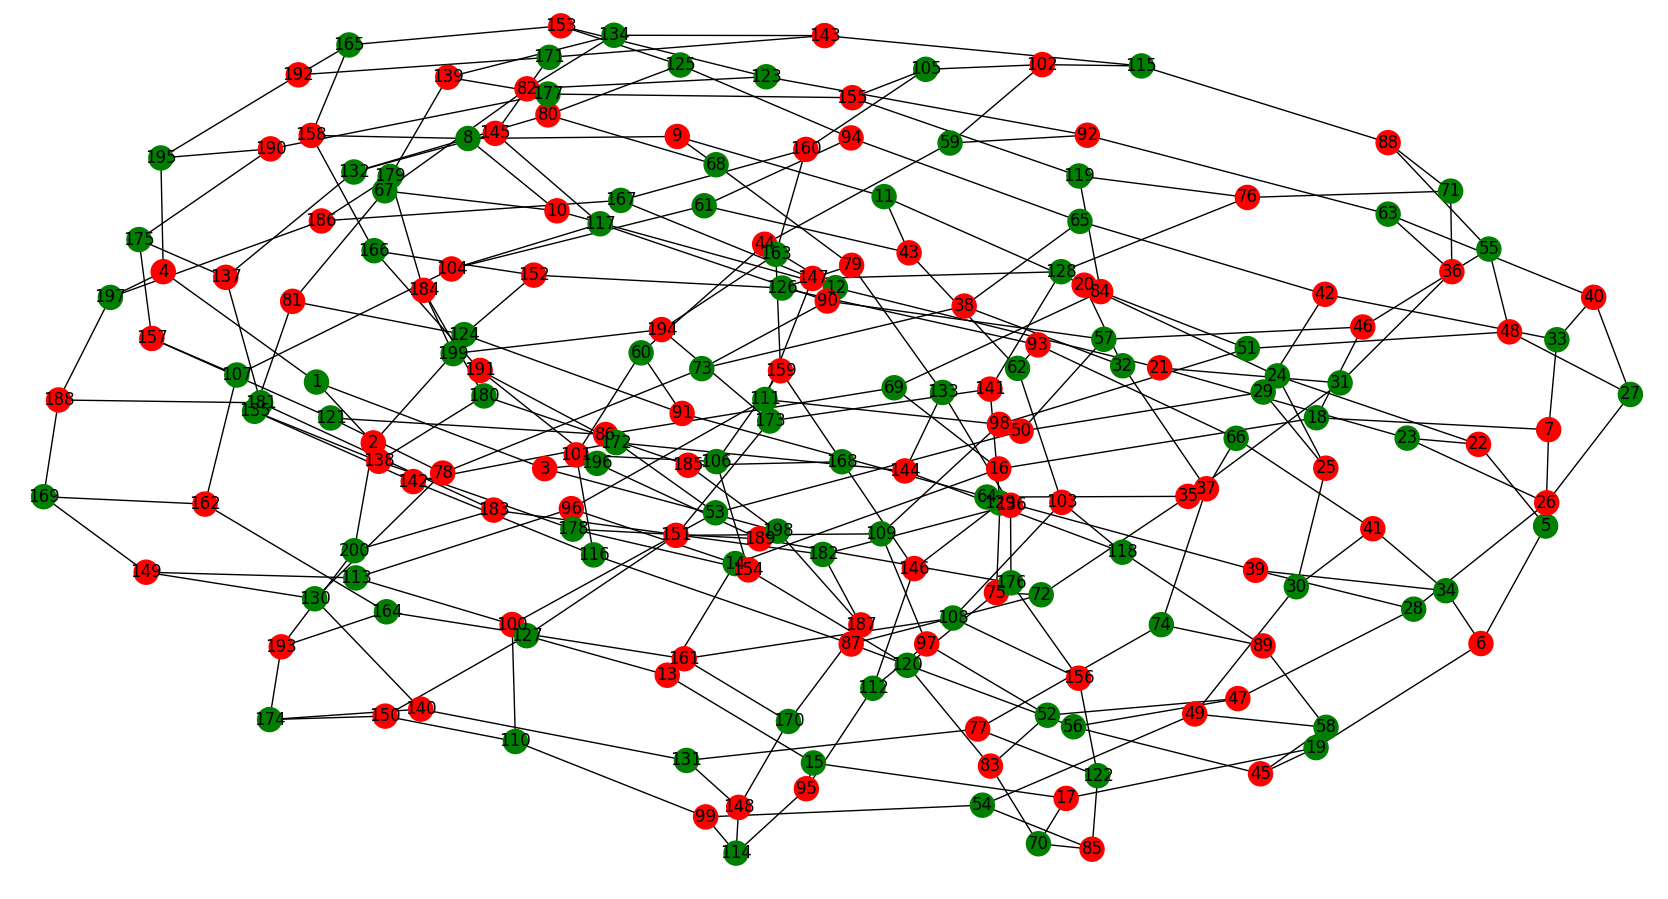
\includegraphics[width=15cm]{images/200_vrhova_bipartitan_graf.png}
\caption{Bojanje bipartitnog grafa s 200 vrhova}
\label{fig:bojanje grafa s 200 vrhova}
\end{figure}

\chapter{Rezultati praktičnog dijela}
Testirane su različite kombinacije parametara i funkcija s ciljem pronalaska optimalnih parametara. Testiranje se provodilo na dva skupa podataka; 200 grafova s rasponom broja vrhova od 1 do 250, te 1226 grafova s rasponom broja vrhova od 200 do 249.

Kao mjera uspješnosti, korištena je \textit{točnost}, omjer broja točno određenih kromatskih brojeva i ukupnog broja grafova za koje se određivao kromatski broj.


\section{Manji skup podataka}
Na manjem skupu podataka od 200 grafova željelo se ustanoviti koliko su algoritmi dobri u pronalaženju rješenja na grafovima s većim rasponom broja vrhova. Pretpostavka je bila da će sve varijacije algoritma biti relativno dobre kod pronalaženja kromatskog broja za jednostavne grafove (mali broj vrhova i bridova), ali da će algoritmi koji koriste slučajan odabir biti lošiji.

Rezultati su podijeljeni po strategiji odabira roditelja, a zatim po strategiji mutacije.

\newpage
\subsubsection{Selekcija stabilnog stanja}
U nastavku su prikazani rezultati algoritama koji koriste selekciju stabilnog stanja za odabir roditelja, uz korištenje različitih strategija mutacije.

\begin{figure}[h]
\centering
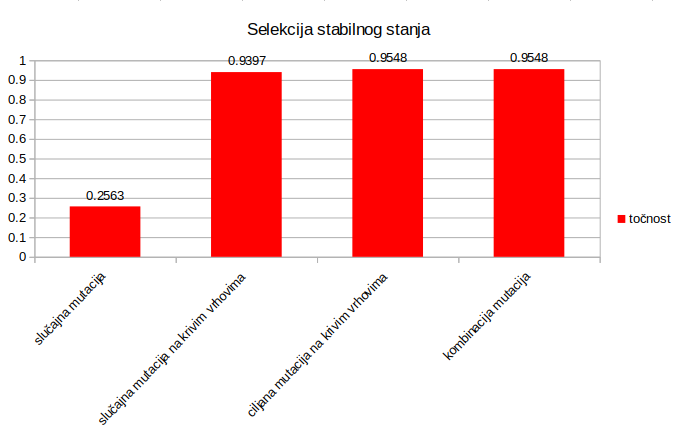
\includegraphics[width=14cm]{images/chart_sss_test_file.png}
\caption{Grafikon točnosti algoritama selekcije stabilnog stanja}
\label{fig:grafikon tocnosti algoritama selekcije stabilnog stanja}
\end{figure}

Iz grafikona sa slike \ref{fig:grafikon tocnosti algoritama selekcije stabilnog stanja} vidimo da je točnost daleko najlošija kod algoritma sa slučajnom mutacijom. Ostale tri varijacije se čine podjednako uspješne, s točnosti od oko 95\%. Slučajna mutacija na krivim vrhovima ima malo nižu točnost od preostale dvije strategije mutacije.

\newpage
\subsubsection{Rang selekcija}
U nastavku su prikazani rezultati algoritama koji koriste rang selekciju za odabir roditelja, uz korištenje različitih strategija mutacije.

\begin{figure}[h]
\centering
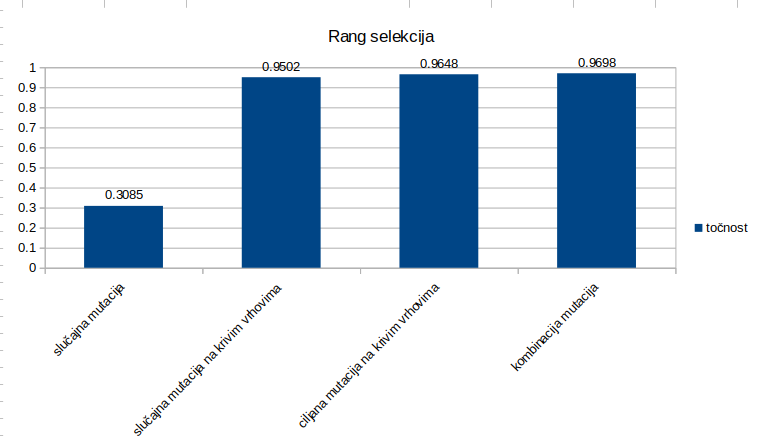
\includegraphics[width=14cm]{images/chart_rank_test_file.png}
\caption{Grafikon točnosti algoritama rang selekcije}
\label{fig:grafikon tocnosti algoritama rank selekcije}
\end{figure}

Kao i kod selekcije stabilnog stanja, iz  grafikona sa slike \ref{fig:grafikon tocnosti algoritama rank selekcije} vidimo da je slučajna mutacija postigla najlošije rezultate. Ostale tri varijacije su podjednako uspješne, s točnosti od preko 95\%. Uspoređujući rang selekciju i selekciju stabilnog tipa, vidimo da je rang selekcija ostvarila bolje rezultate u svakoj od varijacija algoritma.

\newpage
\subsubsection{Slučajna selekcija}
U nastavku su prikazani rezultati algoritama koji koriste slučajnu selekciju za odabir roditelja, uz korištenje različitih strategija mutacije.

\begin{figure}[h]
\centering
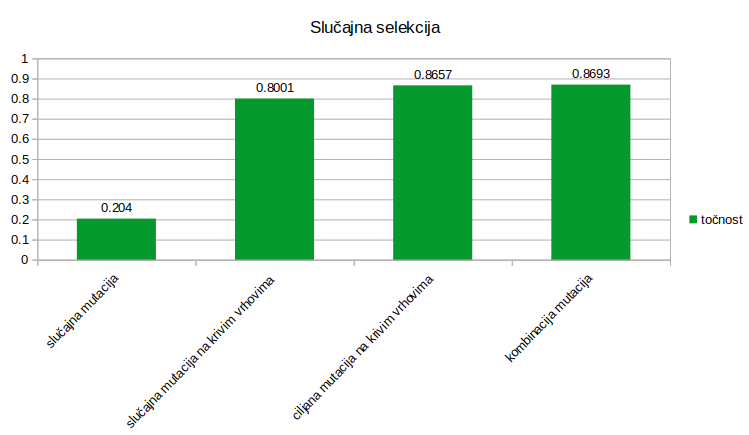
\includegraphics[width=14cm]{images/chart_random_selection_results.png}
\caption{Grafikon točnosti algoritama slučajne selekcije}
\label{fig:grafikon tocnosti algoritama slucajne selekcije}
\end{figure}

Iz grafikona sa slike \ref{fig:grafikon tocnosti algoritama slucajne selekcije} uočavamo da je točnost manja za sve strategije mutacija u odnosu na rang selekciju i selekciju stabilnog stanja. Slučajna mutacija i dalje ima najlošiju točnost od samo 20\%.

\newpage
\subsection{Usporedba rezultata}
U nastavku su prikazane najviše postignute točnosti grupirane po strategijama odabira roditelja.

\begin{figure}[h]
\centering
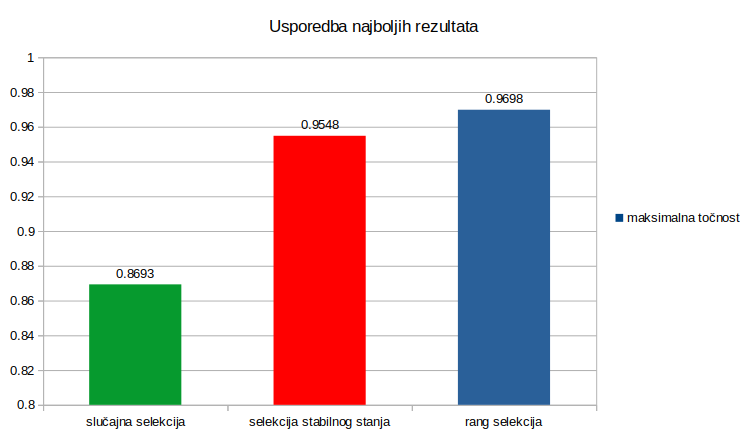
\includegraphics[width=14cm]{images/chart_best_scores.png}
\caption{Grafikon točnosti najboljih varijacija algoritama}
\label{fig:grafikon tocnosti najboljih varijacija algoritama}
\end{figure}

Iz grafikona sa slike \ref{fig:grafikon tocnosti najboljih varijacija algoritama} vidimo da je rang selekcija postigla najbolju točnost, dok je slučajna selekcija najmanje uspješna. Razlika postignute točnosti između te dvije strategije odabira roditelja je čak 10\%. Selekcija stabilnog tipa je vrlo blizu rang selekciji s 95\%-tnom točnošću. 

\newpage
\section{Veći skup podataka}
Na skupu podataka od 1226 grafova s brojem vrhova između 200 i 249 testirane su samo varijacije algoritama koje su ostvarile najbolje rezultate na skupu od 200 podataka.

\subsubsection{Selekcija stabilnog stanja s kombiniranom funkcijom mutacije}

\begin{figure}[h]
\centering
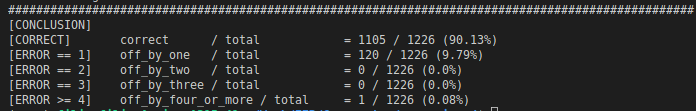
\includegraphics[width=14cm]{images/custom_mutacija_200_249.png}
\caption{Selekcija stabilnog stanja s kombiniranom funkcijom mutacije}
\label{fig:sss kombinirana rezultati}
\end{figure}

Iz rezultata sa slike \ref{fig:sss kombinirana rezultati} vidimo da je algoritam postigao točnost od 90\%. U samo jednom slučaju je pogriješio za 4 ili više, a u preostalim slučajevima je pogriješio za samo jednu boju više.

\subsubsection{Rang selekcija s kombiniranom funkcijom mutacije}

\begin{figure}[h]
\centering
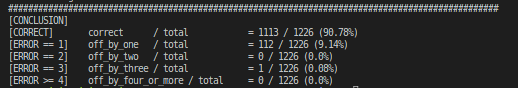
\includegraphics[width=14cm]{images/mutation_func_rank_selection_200_249.png}
\caption{Rang selekcija s kombiniranom funkcijom mutacije}
\label{fig:rank selekcija kombinirana rezultati}
\end{figure}

Iz rezultata sa slike \ref{fig:rank selekcija kombinirana rezultati} vidimo da je algoritam postigao točnost od skoro 91\%. U samo jednom slučaju je pogriješio za 3, a u preostalim je slučajevima pogriješio samo za jednu boju više.

\newpage
\subsubsection{Rang selekcija s ciljanom mutacijom krivih vrhova}

\begin{figure}[h]
\centering
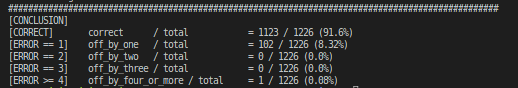
\includegraphics[width=14cm]{images/targeted_change_on_bad_vertices_rank_selection_200_249.png}
\caption{Rang selekcija s ciljanom mutacijom krivih vrhova}
\label{fig:rank selekcija ciljana random rezultati}
\end{figure}

Iz rezultata sa slike \ref{fig:rank selekcija ciljana random rezultati}  vidimo da je algoritam postigao točnost od preko 91.5\%. U samo jednom slučaju je pogriješio za 4 ili više, a u preostalim je slučajevima pogriješio samo za jednu boju više.

\begin{figure}[h]
\centering
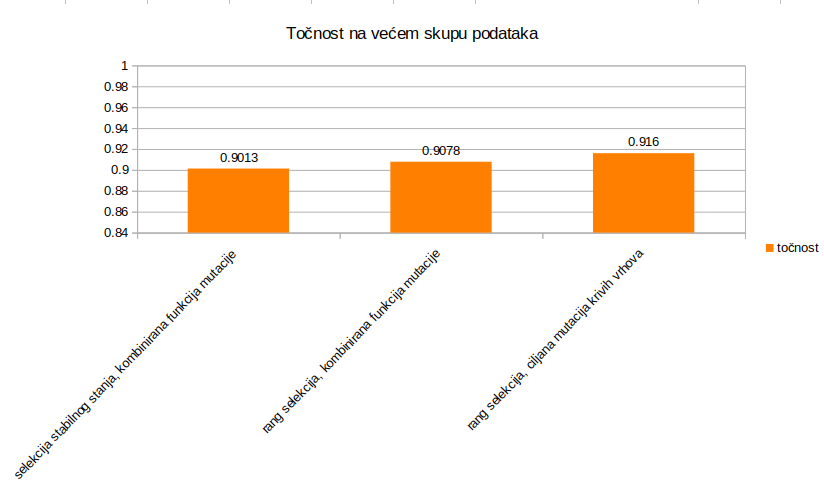
\includegraphics[width=15cm]{images/chart_rezultata_veliki_dataset.png}
\caption{Grafikon točnosti algoritama na većem skupu podataka}
\label{fig:grafikon na vecem skupu podataka}
\end{figure}

Iz grafikona sa slike \ref{fig:grafikon na vecem skupu podataka} vidimo da su točnosti algoritama vrlo blizu. Selekcija stabilnog stanja s kombinacijom funkcija mutacije postigla je najlošiji rezultat, a rang selekcija s ciljanom mutacijom krivih vrhova najbolji.

\chapter{Zaključak}
Dobiveni rezultati ukazuju na uspješnost korištenja genetskih algoritama za rješavanje problema bojanja grafa. Iako nemaju 100\%-tnu preciznost određivanja kromatskog broja, u velikoj većini slučajeva ne griješe za više od jednu boju. 

Kao najbolja kombinacija parametara pokazala se rang selekcija kao strategija odabira roditelja i kombinirana funkcija mutacije ili ciljana mutacija krivih vrhova kao strategije mutacije (slike \ref{fig:grafikon tocnosti najboljih varijacija algoritama}, \ref{fig:grafikon na vecem skupu podataka}). Kombinirana funkcija mutacije pokazala se nešto boljom na manjem skupu podataka, a ciljana mutacija krivih vrhova kao najbolja strategija mutacije na većem skupu podataka.

Mogući razlog uspješnosti ovih strategija je što uz davanje prednosti boljim jedinkama pri razmnožavanju, ciljano mijenjaju gene tako da se oni vrhovi koji su pravilno obojani ne mijenjaju. Strategija selekcije stabilnog stanja nije toliko uspješna jer se po generaciji generira manji broj novih jedinki i na taj način se sporije pretražuje prostor. Budući da je broj iteracija bio limitiran na 1000, takva se strategija nije uspjela proširiti po prostoru dovoljno brzo i pronaći optimalno rješenje.

Najlošije rezultate postigle su strategije koje su se oslanjale na slučajnost (slika \ref{fig:grafikon tocnosti algoritama slucajne selekcije}). Slučajna strategija odabira roditelja pokazala se inferiornijom naspram ostalih strategija biranja roditelja, baš kao i slučajna mutacija gena naspram ostalih strategija mutacije. Razlog je što kod odabira roditelja bolje jedinke nisu dobile prednost, djeca su naslijedila gene od slučajnih roditelja te tako samo rješenje nije konvergiralo prema optimumu. Kod slučajne mutacije gena, problem je što su geni za ovaj specifičan problem unutar jedinki zavisni. Na taj se način moglo dogoditi da su neki već dobro postavljeni geni postali pogrešni, bilo zbog vlastite mutacije ili mutacije susjeda.

Iako su za neke generalne probleme slučajne strategije u sklopu genetskih algoritama korisne, za specifičan problem poput bojanja grafa bolje su se pokazale usmjerene strategije koje uz neku heuristiku ciljano mijenjaju i biraju vrijednosti za sljedeću generaciju.

\bibliography{literatura}
\bibliographystyle{fer}


\begin{sazetak}
U ovom je radu prikazan i opisan način rada evolucijskog algoritma i njegova primjena na rješavanje problema bojanja grafa. Navedene su prednosti i mane pojedinih strategija odabira roditelja i strategija mutacije kod genetskog algoritma. Analiziran je utjecaj različitih strategija na točnost određivanja kromatskog broja grafa te su rezultati međusobno uspoređeni i objašnjeni.

\kljucnerijeci{Evolucijski algoritam, genetski algoritam, kromatski broj, bojanje grafa, strategija mutacije, strategija odabira roditelja}
\end{sazetak}

% TODO: Navedite naslov na engleskom jeziku.
\engtitle{Solving graph coloring problem using evolutionary algorithm}
\begin{abstract}
This paper presents and describes how the evolutionary algorithm works and its application to solving the graph coloring problem. The advantages and disadvantages of individual parent selection strategies and mutation strategies in the genetic algorithm are listed. The influence of different strategies on the accuracy of determining the chromatic number of the graph was analyzed, and the results were compared and explained.

\keywords{Evolutionary algorithm, genetic algorithm, chromatic number, graph coloring, mutation strategy, parent selection strategy}
\end{abstract}

\end{document}

